% Dokumentace k projektu do predmetu GZN
% Autori: David Hromadka
%         Jan Wozniak

\documentclass[a4paper,11pt]{article}
\usepackage[english]{babel}
\usepackage[utf8]{inputenc}
\usepackage[left=1.5cm,text={18cm, 25cm},top=2.5cm]{geometry}
\usepackage{color}
\usepackage[unicode, colorlinks,hyperindex,plainpages=false,pdftex]{hyperref}
\usepackage{graphicx}
\usepackage{float}
\usepackage{multirow}
\usepackage{algorithm}
\usepackage{algorithmicx}
\usepackage{algpseudocode}

\begin{document}

\begin{center}{\LARGE\textbf{Relabel-to-front algoritmus}}\\[0.2cm]
\newcommand{\autor}[2]{#1&\texttt{#2@stud.fit.vutbr.cz}\tabularnewline}
\begin{tabular}{ll}
    \autor{Marek Višňovský}{xvisno00}
    \autor{Jan Wozniak}{xwozni00}
\end{tabular}
\end{center}

\section{Introduction}
This projects purpose was to create simple application for education and visualisation
of Relabel-to-front algorithm. It is implemented purely in Java using Netbeans
IDE.

\section{Theoretical Analysis}
The Relabel-to-front is quite efficient algorithm that computes a maximal flow in
oriented graph. It is a special variant of push-relabel, where the algorithm maintains
list of overflowing nodes. The list is scanned as the algorithm proceeds and the
excess flow in each node is discharged \cite{diz}. 

The main function of the algorithm is \textit{relabel-to-front} which takes three
arguments, graph \textit{G}, source node \textit{s} and sink node \textit{t}\ref{pseud}.
The operation \textit{discharge(u)}\ref{dis} is essential core of the algorithm, 
takes a node \textit{u} and modifies heights and flow in the graph by chosing
suitable push and relabel operations to ensure entire excess flow is taken care of.
If during discharge a node is relabeled, it is moved to the start of the list.
The algorithm then treats the next node in the list and continues the procedure
until every overflowing node has been discharged.
Function \textit{push(u, v)} pushes through edge from node \textit{u} to node
\textit{v} the most excess flow possible. Function \textit{relabel(u)} changes
node's \textit{u} height accordingly.

During initialization height of each node is set to 0 except source, which is set
to \textit{n}. Flow on all edges is set to 0. Then we push the most possible flow
on all edges from source and then continue according to the rest of algorithm\ref{pseud}.

%\begin{algorithm}
%\caption{Relabel-to-front(G,s,t)}
%\begin{algorithmic}
%\If {$i\geq maxval$}
%    \State $i\gets 0$
%\Else
%    \If {$i+k\leq maxval$}
%        \State $i\gets i+k$
%    \EndIf
%\EndIf
%\end{algorithmic}
%\end{algorithm}

\subsubsection*{Computational Complexity}
Every discharge operation without relabel advances $u$, the current 
node within list $L$. Then if we have $n$ discharge operations without relabel,
we have the current node $u = null$ and the algorithm terminates. Therefore, the
number of calls to discharge is at most $n(\#relabels + 1) = O(n^3)$.

A relabel operation at a node is constant time -- increasing label and setting
current-neighbour. In total we have $O(n^2)$.
The cost of push operation is at max $O(n^3)$.

Concluding from the informations above the complexity of relabel-to-front algorithm
is $O(n^3)$ where $n$ is number of nodes \cite{rtf}. 


\section{Implementation}
The program runs in two separate threads, one is GUI and second is relabel to front
algorithm. Entire project is separated into two packages, \texttt{GUI} and \texttt{Graph}.
Graph package contains following classes
\begin{itemize}
\item \textit{Graph} -- basic representation of simple oriented graph
\item \textit{Edge} -- representation of edges
\item \textit{Node} -- representation of nodes
\item \textit{GraphListener} -- interface for communication between UI
\item \textit{RelabelToFront} -- class extending graph of relabel to front algorithm implementation
\end{itemize}

The \texttt{RelabelToFront} stores as protected arrays for flow, capacity, height,
excess and the list of nodes to discharge. The redundant structure is created for
easier reinitialization of algorithm, if the user changes the nodes in graph and
restarts algorithm over again.




\section{User Interface}
Our main goal was to create simple and intuitive, yet powerful user interface. 
We tried to achieve this by minimization of the number of control elements down 
to 2 panels, one for graph building purposes and another one for algorithm control.

\subsubsection*{Creating a simple graph}
Left panel of application's main window serves for graph creation. Users are able 
to add or remove nodes from pop-up menu, that shows up after right click of the 
mouse on the desired location. Nodes are represented as black circles with its 
id displayed inside. Right next to them, there's an indicator of current height 
of the node, which plays role in algorithm itself.

Right clicking on the node invokes the same pop-up menu, but with more options 
enabled, such as deletion of selected node, starting edge from that node, selection 
of this node as source or sink of the graph.

Edges are displayed as lines, with an arrow in the middle pointing in the 
direction of that edge, as relabel-to-front algorithm works with oriented graphs. 
Next to this arrow, there are two numbers separated by slash, indicating current 
flow and capacity of the edge. Edges are created from pop-up menu mentioned above, 
after right clicking on desired start node and then selection of the destination 
node (this is done again by clicking with any mouse button on desired node). 
Loops are not allowed.

\begin{figure}[H]
\centering
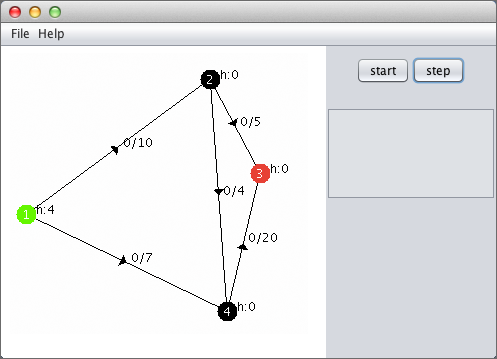
\includegraphics[width=12cm]{1.png}
\caption{Simple graph created in our application. Node 1 is selected as source, node 4 as sink.}
\label{pic1}
\end{figure}

\subsubsection*{Saving and loading graphs}
Application allows to store and load graphs in GraphML format. This is a widely-used 
xml format for graph representation. More info about this format can be found here: 
\url{http://graphml.graphdrawing.org/}. The application can load GraphML files created
by an application itself, other files must contain definition of additional attributes
such as x\_position, y\_position and height for nodes, and capacity for edges. For more
details, look at the saved file itself, the structure is, thanks to xml format, 
easily readable. 

\subsubsection*{Running an algorithm}
To run relabel-to-front algorithm, one must select source and sink nodes first. 
Source node will be colored green and sink node red. After that, users can run 
algorithm simply by clicking on the start button in the panel on the right. 
This will initialize all variables necessary for the algorithm. Then, algorithm 
continues by simple steps after clicking on the step button. Changes to the 
graph are highlighted:
\begin{itemize}
\item node, which turns yellow, had its height changed in the last step (height 
number turns to red)
\item edge, which flow has changed, is highlighted by yellow border, and its 
flow and capacity marking is written in red
\end{itemize}

There are steps of the algorithm, when relabel-to-front works with virtual edges,
which are not visible to the user. Information about these changes (and also 
about all visible changes) can be found in text area below the control buttons.
Final flow is displayed here too.

\begin{figure}[H]
\centering
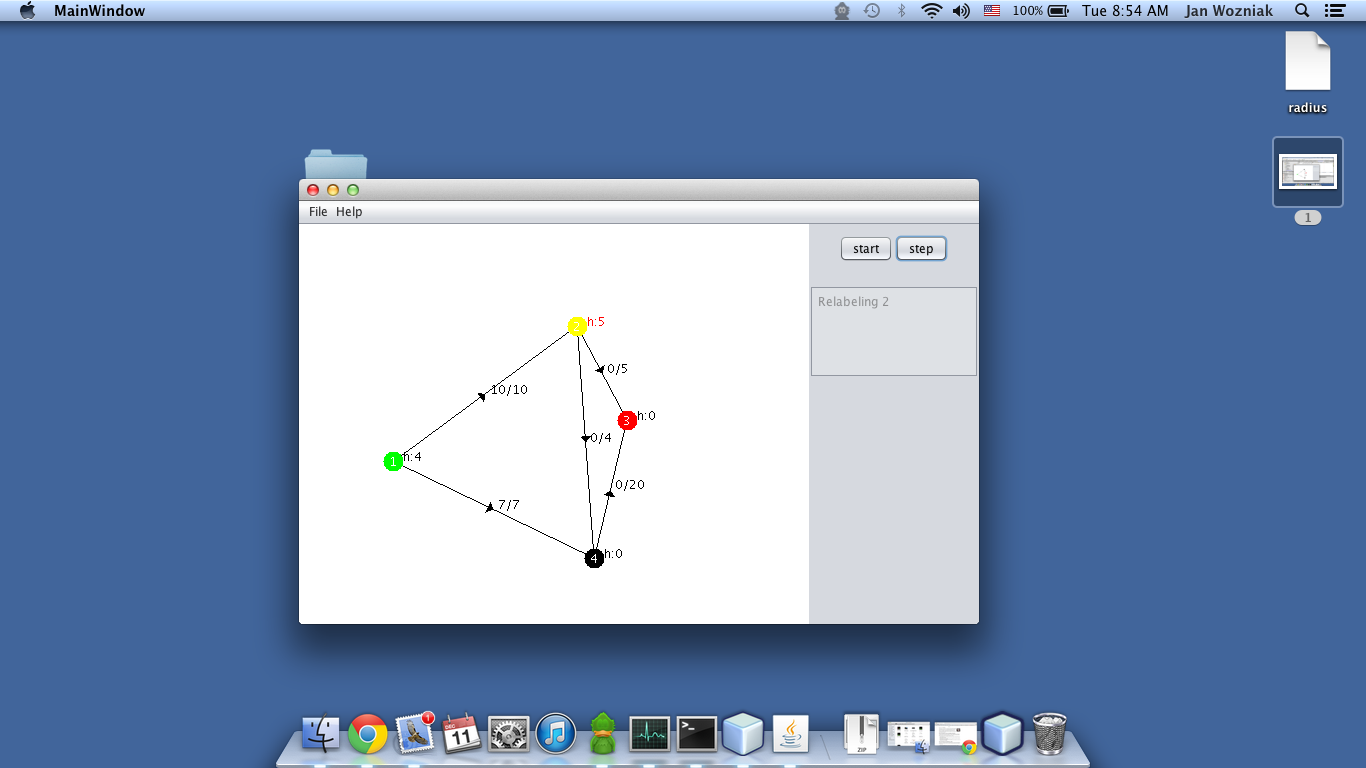
\includegraphics[width=12cm]{2.png}
\caption{Running an algorithm. Node 2 is being relabeled, so it is painted in yellow.}
\label{pic1}
\end{figure}

\section{Conclusion}


%
%
% LITERATURA
% ======================
\newpage
{%
    \renewcommand{\refname}{Literature} % Text nadpisu thebibliography.
    \newcommand{\bi}[5]{\bibitem{#1}{#2}\textit{#3.} #4\\{}$<$\url{#5}$>$}%
    \newcommand{\citdatum}[1][2011-10-08]{$[$cit.~{#1}$]$}%
%
\begin{thebibliography}{MM}%
% Vzor: \bi{label}{Název}{Poznámky.}{http://www.adresa.cz/}%
\bi{diz}{A. Bhusnurmath. }{Applying Convex Optimization Techniques to Energy Minimization Problems in Computer Vision}{\citdatum[2012-12-11]}
    {http://www.cis.upenn.edu/~cjtaylor/PUBLICATIONS/pdfs/BhusnurmathPHD08.pdf}
\bi{rtf}{E. Mayr, H. Räcke. }{Relabel to front -- Lecture}{\citdatum[2012-12-10]}
    {http://wwwmayr.informatik.tu-muenchen.de/lehre/2011WS/ea/split/sub-Relabel-to-front-single.pdf}

\end{thebibliography}}
\end{document}
